\section{Results}\label{sec:results}

\subsection{Agent Type}\label{subsec:agent-type}
The average rewards by agent type can be seen in \autoref{fig:rewards-by-agent}.
Unfortunately, none of the agents were able to do as well as the controller used by the
CPT\@.
Additionally, all agents performed as bad or worse as a simple random controller!
It is possible that this problem is complex enough that the models needed more time
to train, but no significant additional gains were made when training for over 12,000
episodes, so there appears to be something wrong.

\begin{figure}[!ht]
    \centering
    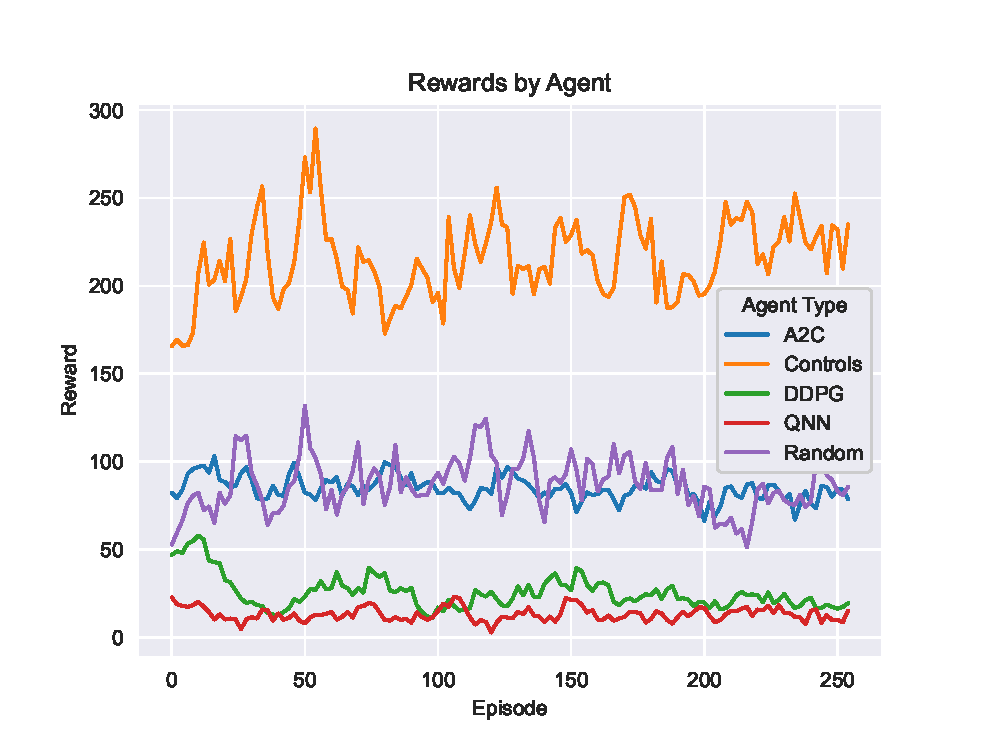
\includegraphics[scale=0.5]
    {./figures/rewards-by-agent}
    \caption{
        Rewards by agent type achieved during the testing phase of each episode.
        The x-axis is the episode, while the y-axis is the reward.
    }
    \label{fig:rewards-by-agent}
\end{figure}

Interestingly, the A2C agents seems to perform the best out of all the agents used.
DDPG seems to perform second best, while QNN performs the worst.
Further work should be done to determine why these agents aren't improving and what
changes need to be made to improve them.
The average reward for each agent is shown in \autoref{tab:agent-average-reward}.

\begin{table}[!htbp]
    % increase table row spacing, adjust to taste
    \renewcommand{\arraystretch}{1.3}

    \caption{The average rewards by agent type.}
    \label{tab:agent-average-reward}

    \centering
    \begin{tabular}{|c|c|}
        \hline
        Agent    & Average Reward \\
        \hhline{|=|=|}
        A2C      & 84.77          \\
        \hline
        Controls & 216.75         \\
        \hline
        DDPG     & 25.05          \\
        \hline
        QNN      & 13.04          \\
        \hline
        Random   & 87.68          \\
        \hline
    \end{tabular}
\end{table}

\subsection{Memory Type}\label{subsec:memory-type}
The loss by memory type is displayed per agent type in \autoref{fig:loss-by-memory}.
Specifically, the loss for the actor is used in the case of A2C and DDPG, while QNN
simply displays ``loss'' since it itself is the actor.

\begin{figure}[!ht]
    \centering
    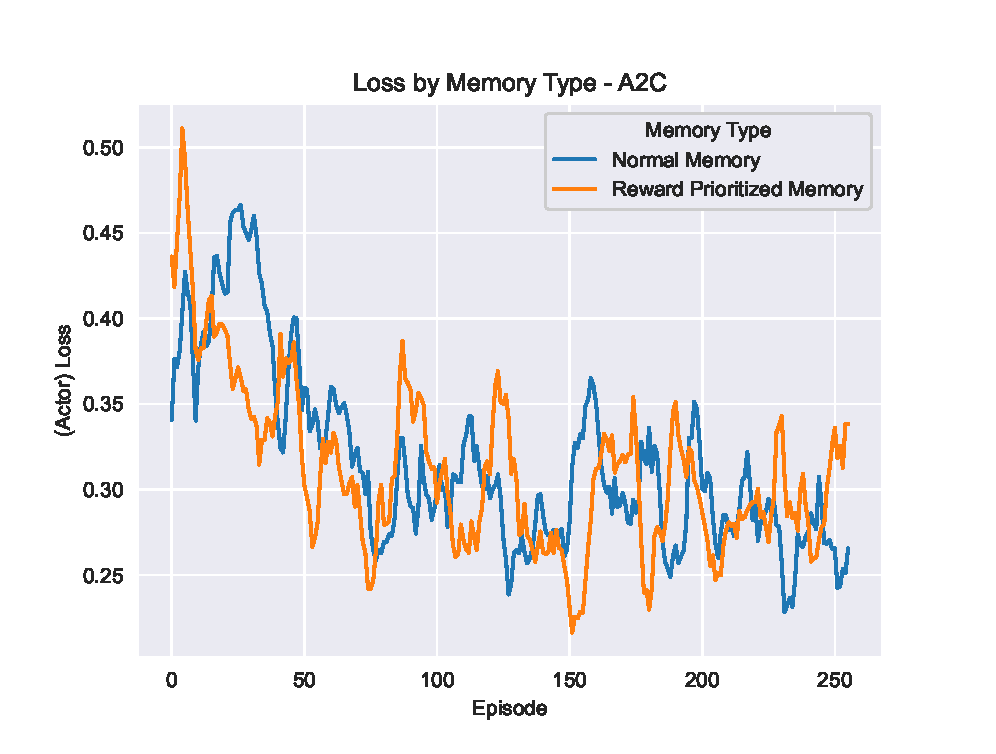
\includegraphics[scale=0.5]
    {./figures/memory/loss-by-memory-A2C}
    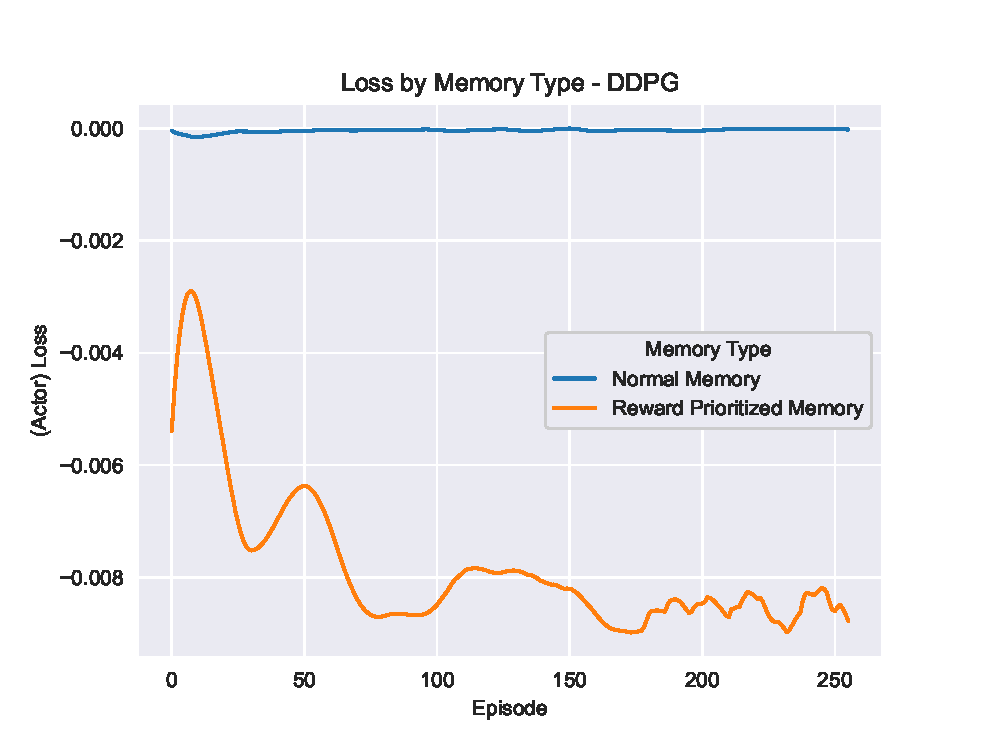
\includegraphics[scale=0.5]
    {./figures/memory/loss-by-memory-DDPG}
    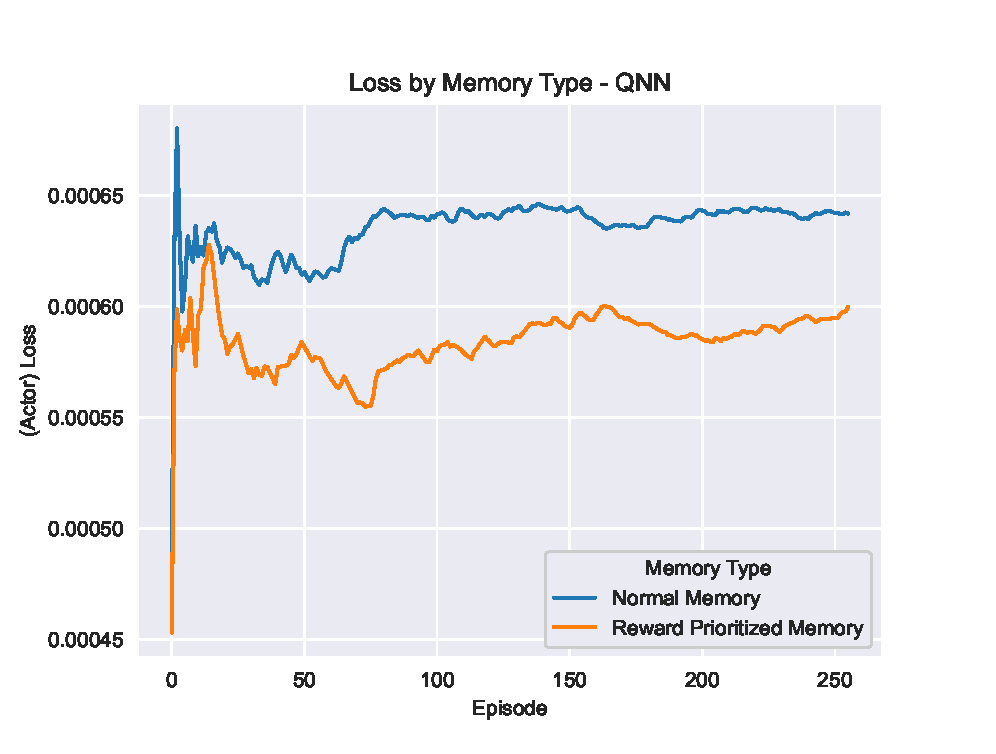
\includegraphics[scale=0.5]
    {./figures/memory/loss-by-memory-QNN}
    \caption{
        Loss by memory type for each agent type per episode.
        The x-axis is the episode, while the y-axis is the loss.
        Lower loss is better than higher loss.
    }
    \label{fig:loss-by-memory}
\end{figure}

RPM initially appears to provide better gains in terms of loss.
Specifically, there is an initial dip in loss, but then the slopes of RPM and normal
memory seem to converge.
DDPG especially seems to gain a huge benefit from RPM, but it should be noticed that
for all agents the advantage provided by RPM is fairly small, typically only
consisting of hundredths of decimal places, if that.
Additional experiments should be performed to confirm the effectiveness, or lack
thereof, of Reward Prioritized Memory.

\subsection{Architecture}\label{subsec:architecture}
The rewards for each architecture can be seen in
\autoref{fig:rewards-by-architecture}, which includes both types of networks as well
the same networks with LSTM layers injected before the output.
The average reward for each architecture is additionally tabulated in
\autoref{tab:architecture-average-reward}.

The simple networks include a series of linear layers with LeakyReLu activation
functions.
The distance networks use a series of convolutional layers on the distance
observations before passing their results to the rest of the network.

\begin{figure}[!ht]
    \centering
    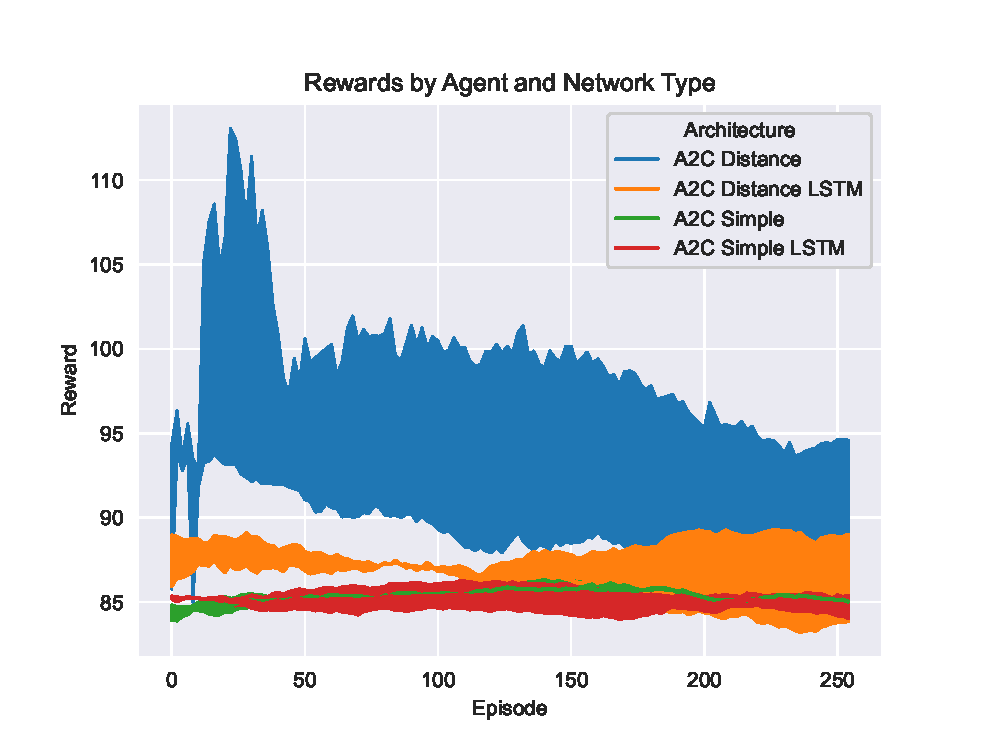
\includegraphics[scale=0.5]
    {./figures/architecture/rewards-by-architecture-A2C}
    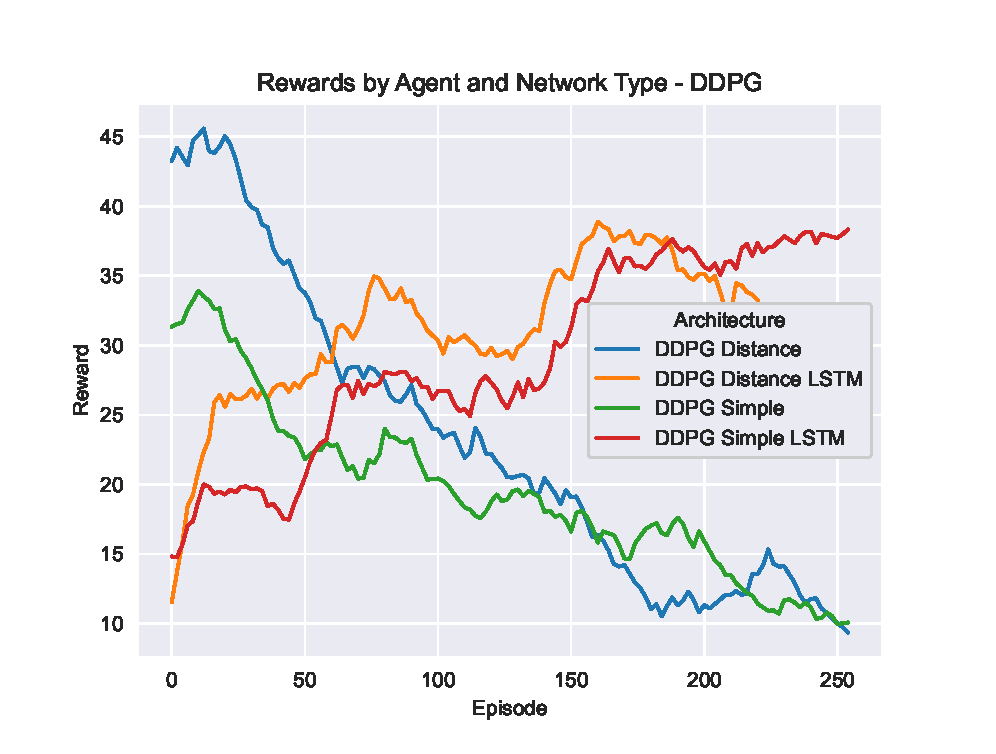
\includegraphics[scale=0.5]
    {./figures/architecture/rewards-by-architecture-DDPG}
    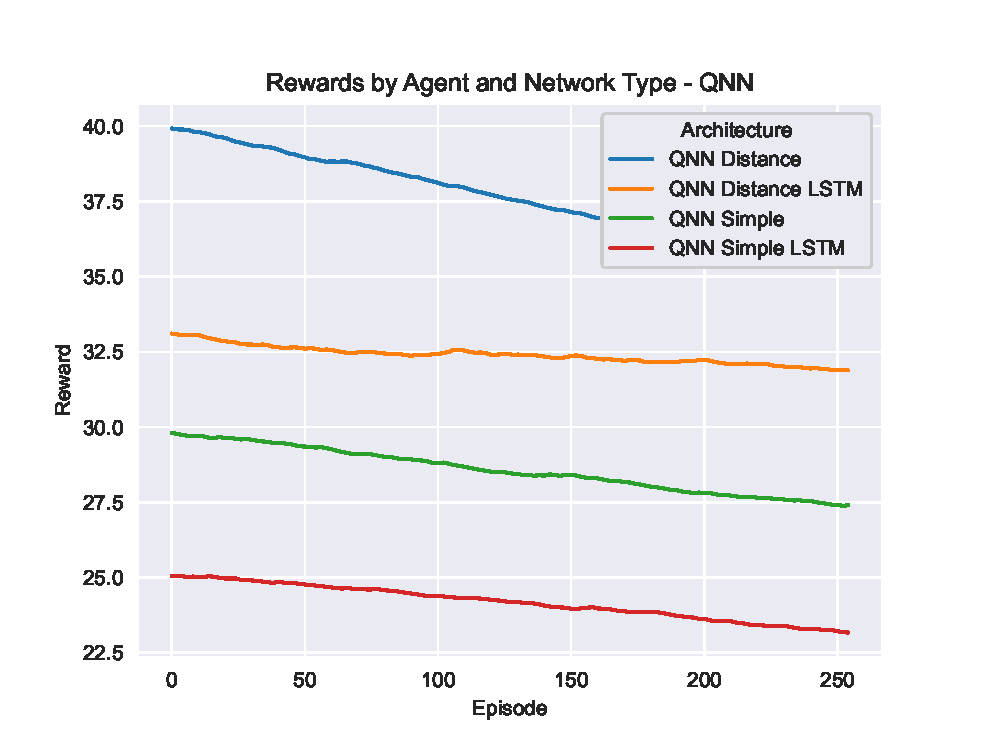
\includegraphics[scale=0.5]
    {./figures/architecture/rewards-by-architecture-QNN}
    \caption{
        Rewards by architecture type for each agent type from the testing phase for
        each episode.
        The x-axis is the episode, while the y-axis is the reward.
        Those architectures with LSTM contain a LSTM layer before the output layer.
    }
    \label{fig:rewards-by-architecture}
\end{figure}

Interestingly, the distance networks consistently perform better than the simple
networks.
A2C in particular benefited from distance networks.
This is not too surprising, since the convolutional layers would allow the network to
extract additional features from what the agent ``sees.''
What is surprising is the LSTMs consistently performed \textit{worse} than the
non-LSTM equivalents.
This is strange because the LSTMs should allow the agent to better recognize the time
element of Waterworld, and yet the consistently underperformed.
It is possible they needed additional time to train, since they add an additional
level of complexity.

\begin{table}[!htbp]
    % increase table row spacing, adjust to taste
    \renewcommand{\arraystretch}{1.3}

    \caption{The average rewards by architecture type.}
    \label{tab:architecture-average-reward}

    \centering
    \begin{tabular}{|c|c|c|}
        \hline
        Agent Type & Network Type       & Average Reward \\
        \hhline{|=|=|=|}
        A2C & Distance       & 86.61          \\
        \hline
        A2C & Distance LSTM  & 82.85          \\
        \hline
        A2C & Simple         & 87.26          \\
        \hline
        A2C & Simple LSTM    & 82.36          \\
        \hline
        DDPG & Distance      & 14.53          \\
        \hline
        DDPG & Distance LSTM & 35.86          \\
        \hline
        DDPG & Simple        & 14.30          \\
        \hline
        DDPG & Simple LSTM   & 35.51          \\
        \hline
        QNN & Distance       & 7.19           \\
        \hline
        QNN & Distance LSTM  & 23.79          \\
        \hline
        QNN & Simple         & 10.98          \\
        \hline
        QNN & Simple LSTM    & 10.18          \\
        \hline
    \end{tabular}
\end{table}

\subsection{DDPG with CPT}\label{subsec:ddpg-with-cpt}
This section examines pretraining a DDPG critic using a Controls Policy Trainer.
Both DDPG agents trained use the same architecture: a distance neural network using
convolutional layers with a simple linear critic.
The only difference is the CPT DDPG receives a pre-trained critic.
This critic continues to train with the actor so the agent is eventually able to
perform better than the CPT\@.
However, it is possible to freeze the critic or even temporarily freeze the critic
until the actor performs similarly to the controller.

As seen in \autoref{fig:cpt-graphs}, the CPT DDPG may have advantages over the normal
DDPG\@.
In particular, the loss of the actor starts with a significant dip in loss.
However, it then proceeds to oscillate around the normal DDPG loss, which may not be
desirable.
This may be because the DDPG CPT actor is encountering situations the Trainer had not
encountered, since the Trainer uses a fairly simple controller.

\begin{figure}[!ht]
    \centering
    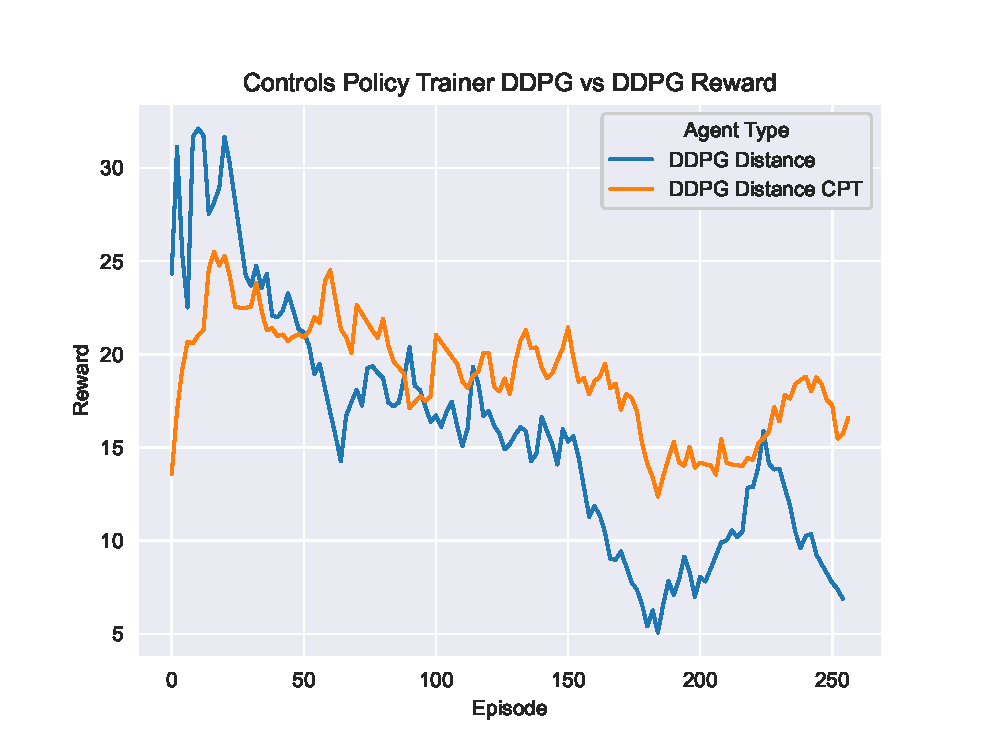
\includegraphics[scale=0.5]
    {./figures/cpt/rewards-by-agent-cpt}
    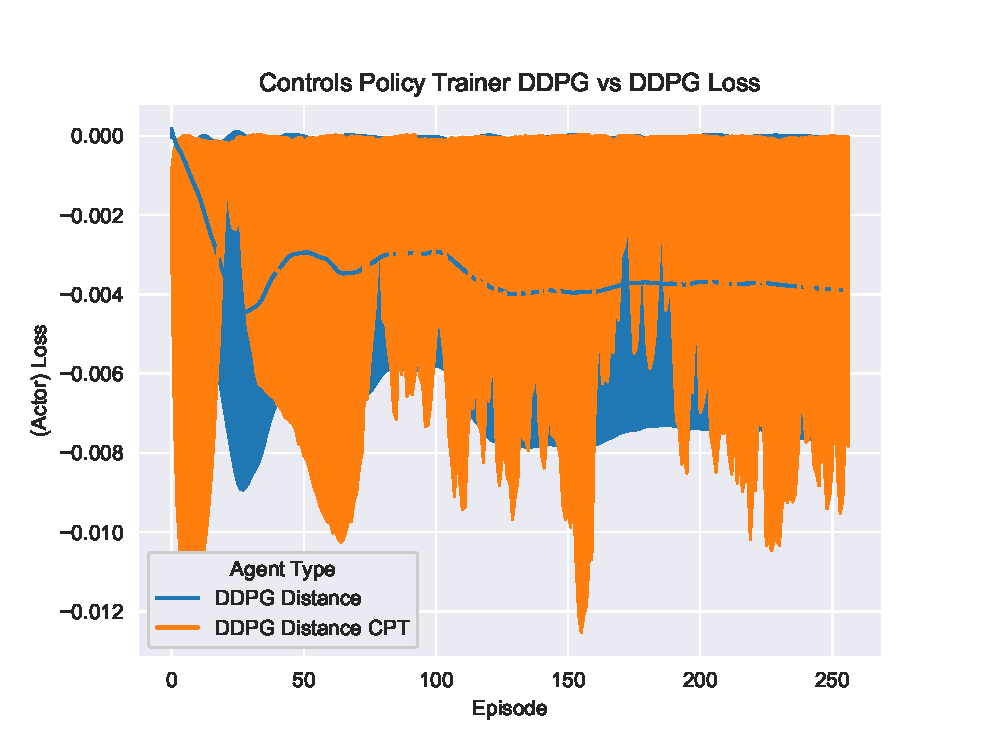
\includegraphics[scale=0.5]
    {./figures/cpt/loss-by-agent-cpt}
    \caption{
        \textbf{Top:} Rewards for DDPG vs DDPG with CPT per training episode during
        test phase.
        \textbf{Bottom:} Actor loss for DDPG vs DDPG with CPT per training episode
        during test phase.
    }
    \label{fig:cpt-graphs}
\end{figure}

This technique in particular may be promising and should be further researched.
By pretraining a strong policy/critic, one can rapidly develop agents and determine
the best architecture to use for the actor.
